\documentclass{article}
\usepackage{cite}
\usepackage{graphicx}
\begin{document}

\section{Top PLDs of entity sources}

\begin{figure}[!tbp]
  \caption{Top Pay-Level Domains (PLDs) of entities in BTC-2009}
  \centering
  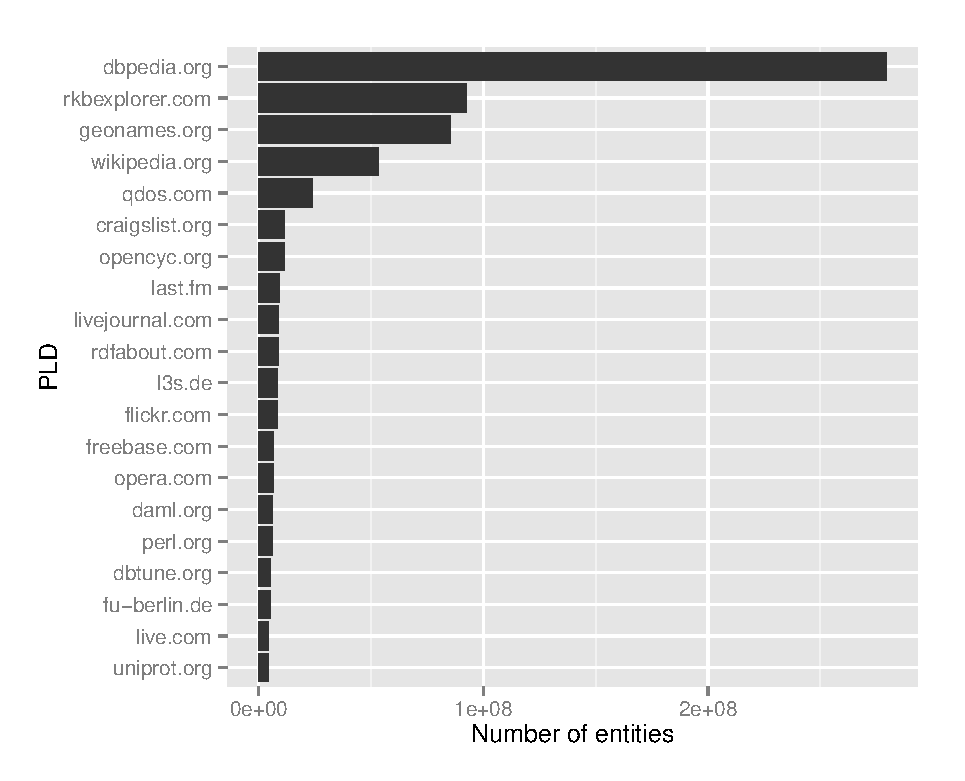
\includegraphics[width=0.7\textwidth]{../btc-2009}
  \label{fig:btc2009}
\end{figure}
\begin{figure}[!tbp]
  \caption{Top Pay-Level Domains (PLDs) of entities in BTC-2012}
  \centering
  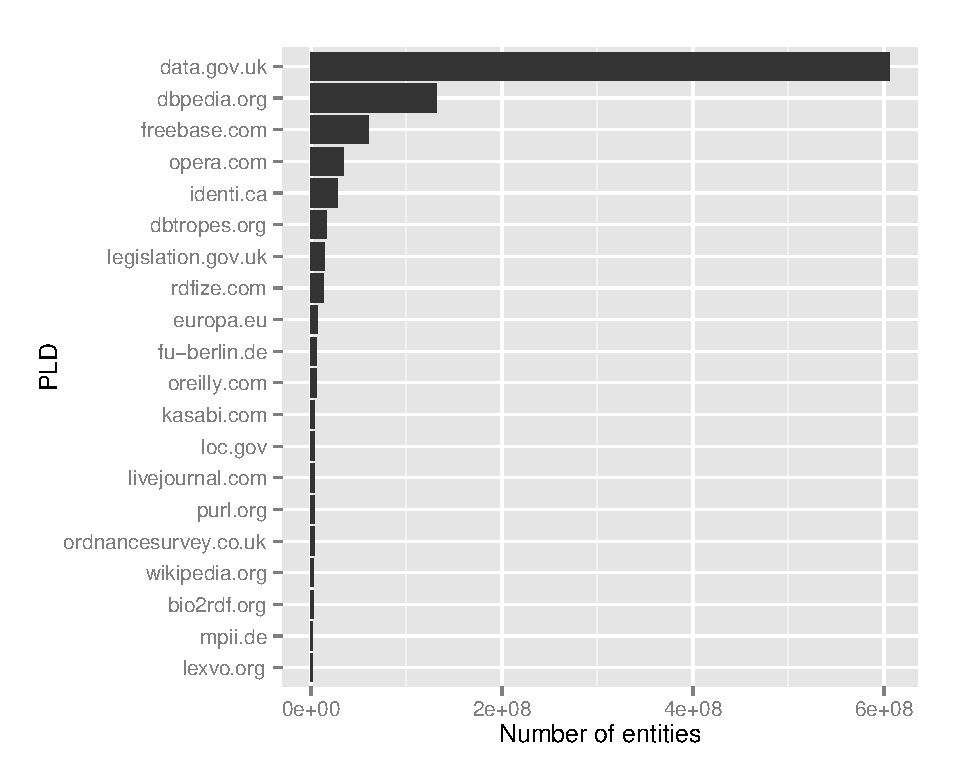
\includegraphics[width=0.7\textwidth]{../btc-2012}
  \label{fig:btc2012}
\end{figure}
\begin{figure}[!tbp]
  \caption{Top Pay-Level Domains (PLDs) of relevant entities in Semantic Search
    Challenge 2010/2011}
  \centering
  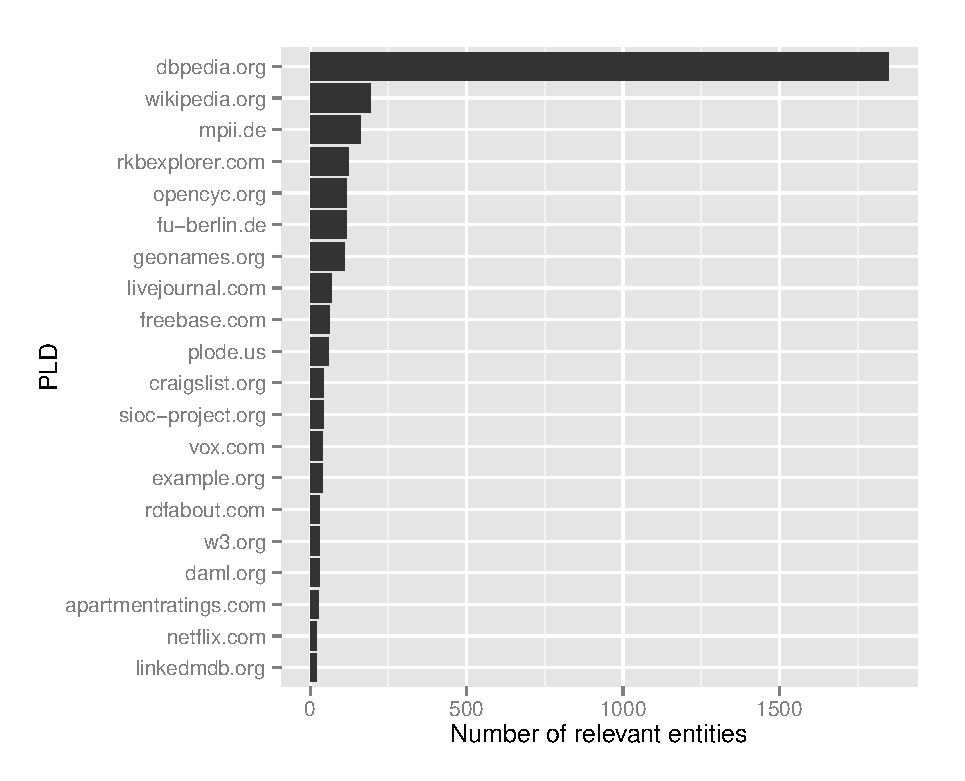
\includegraphics[width=0.7\textwidth]{../relevant}
  \label{fig:relevant}
\end{figure}

Figures~\ref{fig:btc2009}, \ref{fig:btc2012} and \ref{fig:relevant} show numbers
of entities for Top-20 Pay-Level Domains for the whole BTC-2009 and BTC-2012
datasets as well as for relevant results from SemSearch Challenge judgments
only. It can be observed that in BTC-2009 dataset entities are significantly
skewed towards DBpedia, and for SemSearch Challenge this disproportion is even
higher as was noted in \cite{balog2013test}. In BTC-2012 DBpedia became the
second most popular source for entities following datasets from data.gov.uk.
Speaking of numbers, in the whole BTC-2009 dataset DBpedia entities constitute
$34.6\%$ of all entities and in relevance judgments they constitute $48.9\%$ of
all relevant results. In BTC-2012 DBpedia entities constitute only $13.6\%$ of
all entities, while data.gov.uk entities constitute $62.6\%$.

% Starting from BTC-2012 \cite{btc-2012} the problem was mostly solved as can be
% seen in \cite{btc-2012-stats}

\section{Feature usefulness analysis}

We've analyzed significance of our features for different types of concepts
using one-sided Mann-Whitney test (significance level $= 0.01$). We've observed
that for Field Probability feature for concepts of type \emph{attribute} values
of feature for \emph{attributes} field are significantly higher than values for
all three names fields (\emph{names}, \emph{similar entity names}, and
\emph{related entity names}); for \emph{entity} and \emph{relation} concept
types feature value for all names fields is significantly higher than values for
both \emph{attributes} and \emph{categories} fields; for \emph{type} concepts
Field Probability values for \emph{categories} field is significantly higher than values
for all other fields. For Top Score feature values for \emph{attribute} concepts
for \emph{attributes} field is higher than values for all other fields; for
\emph{relation} concepts values for \emph{similar entity names} are
significantly higher than values for all other fields.

\bibliography{desc}{}
\bibliographystyle{plain}
\end{document}